

Bakgrund teori om cellen
\begin{itemize}
    \item Cytoplasmans uppbyggnad och struktur
    \item Brownsk rörelse, CTRW, Fractional Brownian motion
    \item Metabola tillståndets påverkan på partikelrörelsen
\end{itemize}
Bakgrund för dataanalysen
\begin{itemize}
    \item Anisotrop miljö
    \item Skillnad mellan energydepleted och logphase (för alla nedan)
    \item Radius of gyration = Rörlighet
    \item MSD(vilken modell passar bäst)
    \item Korrelationsfunktioner
\end{itemize}


%%%%%%%%%%%%%%%%Riktig text nedan%%%%%%%%%%%%%%%%%%%%%

\section{Teori}
\todo[inline]{Inga tomma rubriker.}

\subsection{Jästceller}
Miljontals år av evolution har lett till att det idag finns en mängd
olika sorters celler med sina enga inre strukturer. %Kanske lite väl brett?
Det finns allt från bakteriers tillsynes oordnade inre till
djurcellers högst strukturellt ordnade innanmäte. Datan som detta
arbete bygger på kommer från observationer av partikelrörelse i
jästceller. 

Jäst~\cite{SGD_yeast} hör till riket svampar och utgörs av encelliga
organismer.  Att den är en encellig organism möjliggör snabb
reproduktion vilket gör den smidig att arbeta med i
laboratorium. Dessutom uppvisar de större likhet med  djurceller än de
likväl encelliga bakterierna och ger därmed större möjlighet för att i
försök på jästceller dra paralleller till djurceller. 


\subsection{Jästcellers cytoplasma}
Att jästceller är svampar innebär att de därmed varken är djur, växter
eller bakterier men delar vissa likheter med de alla tre. Med sitt
arvsanlag samlat i en cellkärna~\cite{SGD_yeast}, precis som djur- och
växtceller, 
%(karakteristiskt för eukaryoter) 
skiljer sig jästceller från bakterier där arvsanlaget ligger blandat
med resten av beståndsdelarna i cytoplasman.
%(karakteristiskt för prokaryoter). 
De har även en vakuol och stabiliserande cellvägg som växtceller men
saknar växtcellens kloroplaster och kan därmed inte utföra någon
fotosyntes.


Djurcellernas komplicerade nät av proteintrådar, som möjliggör en aktiv
transport inom cellen, finns inte hos jästceller som istället får
förlita sig på passiv transport, förutom vid just
celldelning. \todo{Källa?} 
Med jästceller kan man därför undersöka om anomalier från Brownsk
rörelse uppkommer även utan de 
\todo{Hur stokastiska är motorproteinens krafter?} 
stokastiska krafter som har sitt ursprung i motorproteinernas bidrag
till partiklarnas förflytning.

\todo[inline]{Jag skulle vilja få en lite mer utvecklad förklaring av
  motorproteinen (vad/hur de gör). Kanske hade varit en bra idé att ha
  ett litet större avsnitt (eller eget kapitel) om celler innan vi
  börjar prata om partiklar och strängar.}
  \todo{Frågan är hur mycket vi bör uttala oss om motorprotein då dessa inte är aktiva under våra mätningar}

\subsubsection{Metabola tillståndets påverkan på partikelrörelsen}
Jästceller har förmågan att kunna gå i dvala, ett tillstånd där de
intracellulära aktiviteterna minskar. Då delar av den tillhandahållna
datan kommer från celler i dvala möjliggör detta undersökningar om
huruvida cytoplasmans beståndsdelars rörlighet i cellen beror på
cellens metabola tillstånd. 

Tidigare studier~\cite{Gou_etal2014} på eukaryota celler har visat att
partiklars rörlighet i cytoplasman beror på hur aktiv cellen
är. Rörligheten i de undersökta cellerna ökade exempelvis
trefaldigt om cellen drabbats av cancer jämfört med en normalt
fungerande cell. En cell som drabbats av cancer kommer att ha en
förhöjd metabolism för att öka på celldelningstakten. Den sammanlagda
påverkan av motorproteinerna utpekas i dessa studier
\todo{Vilka studier? Är det Gou eller Parry?} 
som en möjlig kandidat till fenomenet. 

Studier~\cite{Parry_etal2014} på bakterier har samtidigt visat att
partiklarnas rörlighet minskade drastiskt om den metabola aktiviteten
minskade. Då bakterier saknar aktiv transport i sina celler försökte
\todo{Är det Parry?} man här istället nå en förklaring via att
cytoplasman blir mer vätskelik ju högre aktiviteten är och börjar
likna ett mer elastiskt fast material då aktiviteten
minskar. Partikelstorleken tycks också vara en faktor för dess förmåga
att röra sig runt i cellen. I gränsen när partiklarna närmar sig
storleken av organellerna i cytoplasman blir förklaringen uppenbar;
partikeln kommer då på grund av sin storlek inte att kunna röra sig
runt i cellen som vid fri diffusion. 


\section{Modeller för rörelse i cytoplasman}
\todo{Detta stycket skulle t.ex. kunna sägas i kapitlet om celler i
  stället.}
I celler talar man om två typer av transport: den aktiva och den
passiva transporten. Under den aktiva transporten vandrar motorprotein
längs med proteintrådar och för med sig det som ska transporteras.
% under användande av kroppens energikälla ATP. 
Under den passiva transporten tillåts ämnena diffundera fritt genom
cytoplasman. Vilket transportsystem som är dominerande beror på vilken
celltyp man betraktar. Jästceller har, som beskrivet ovan, endast
passiv transport mellan celldelning. Så detta arbete kommer att
fokusera på just passiv transport, det vill säga diffusion av partiklar. 

Till en första approximation skulle rörelsen för en partikel i cytoplasman kunna beskrivas med klassisk Brownsk rörelse där partiklarna krockar med mindre partiklar från omgivningen och där rörelsen kan beskrivas med en stokastisk gaussisk propagator. Denna teori bygger dock på att man har termisk jämvikt och att partiklar rör sig i en helt viskös vätska, två kriterier som inte uppfylls i cytoplasman bland annat på grund av mitokondriernas energiutvinning. Andra modeller måste sålunda tillämpas för att nå en bättre beskrivning. Två kandidater är ''Continuous Time Random Walk'' (CTRW) och ''Fractional Brownian motion''.

\todo[inline]{Se över vad som kan tas bort nu när det finns ett eget
  kapitel om stokastik.}

\subsubsection{Brownsk rörelse} \label{sec:Brownsk}
Hastigheten för en partikel som utför ren Brownsk rörelse styrs av
Langevinekvationen~\cite{Mazo_Brownian2002} \todo{Föklara Langevin.}
\begin{equation} %\label{eq:Brownian_SDE}
    M\dv{v}{t}=-\zeta v + F(t),
\end{equation}
där $M$ är partikelmassan, $\zeta$ en friktionskonstant och $F(t)$ en
fluktuerande kraft. Kraften utgör här det stokastiska bidraget till
differentialekvationen och är deltakorrelerat i tiden,
$\ev{F(t)F(t')}=\sigma^2\delta(t-t')$, 
med väntevärde 0, $\ev{F(t)}=0$. 
Det vill säga att den beter sig som vitt brus. 

Den fysikaliska tolkningen av denna stokastiska kraft är att partikeln får små impulser från omgivande vätskepartiklar vilka kolliderar slumpmässigt med den brownska partikeln.  Deltakorrelationen för kraften uppkommer då impulserna modelleras som deltafunktioner i tiden. Denna kraftterm kan vidare tolkas som derivatan av en Wienerprocess i gränsen då kollisionerna infaller med hög frekvens. En Wienerprocess är en tidskontinuerlig stokastisk process där varje förändringssteg är oberoende av tidigare steg samtidigt som \todo{Bättre ord än ökningar}ökningarna är normalfördelade med väntevärde 0..
%Motivation att derivata av Wienerprocess s63

Lösningen till den stokastiska differentialekvationen \eqref{eq:Brownian_SDE} ges av \todo{Vill vi ändra till 2D?}
\begin{equation}
    v(t)=v(0)e^{-\nicefrac{\zeta t}{M}}+\frac{1}{M}\int^t_0 F(s)e^{-\nicefrac{\zeta (t-s)}{M}}ds.
\end{equation}
Detta får dock inte den stokastiska termen att försvinna och lösningen kan inte skrivas på en deterministisk form. För att ändå kunna göra några förutsägelser kan man titta på väntevärdet och korrelationen i tiden.

För $t \gg \nicefrac{\zeta}{M}$ blir $\nicefrac{\dd{v}}{\dd{t}}$-termen i ekvation \eqref{eq:Brownian_SDE} försumbar \todo{Visa detta?} och ekvationen kan då skrivas på formen
\begin{equation}
    \zeta \dv{x}{t}=F(t),
\end{equation}
där $x$ är partikelns position. Detta ger lösningen
\begin{equation}
    x(t)=x(0)+\frac{1}{\zeta} \int^t_0 F(s)ds.
\end{equation}
Utifrån denna lösning kan medelvärdet av den kvadrerade avvikelsen beräknas, kallat ''mean squared displacement'' (MSD), vilken blir 
\begin{equation} \label{eq:MSD_Brownsk}
    \ev{(x(t)-x(0))^2}=\frac{2k_BTt}{\zeta}
\end{equation}
där fluktuation-dissipationsteoremet gett att $\sigma^2=2k_BT\zeta$. \todo{ska vi visa flukt.diss.teoremet?} MSD:n kommer därmed att öka linjärt med tiden, något som enkelt kan jämföras med uppmätt data.



\subsubsection{Continuous Time Random Walk (CTRW)}
En möjlig förklaringsmodell för anomal transport\todo{Förklara varför
  anomal transport ens är intressant att studera.}
i celler utgörs av CTRW (continuous-time random
walks)\cite{Hofling&Franosch2013}. Här beskrivs rörelsemönstret av att
partiklarna under majoriteten av tiden sitter bundna till olika
strukturer för att sedan plötsligt ta sig vidare till en ny position
efter en viss väntetid, där positionsändringen och väntetiden beskrivs
av en stokastisk variabel. Anomal transport uppkommer här genom att
medelväntetiden mellan två hopp blir oändlig och därmed att centrala
gränsvärdessatsen ej uppfylls. Summan av de stokastiska variablerna
går således ej mot att bli normalfördelad, något som är grundläggande
i teorin kring Brownsk rörelse. 

\subsubsection{Fractional Brownian Motion}

En annan modell som kan undersökas är Fractional Brownian motion~\cite{Hofling&Franosch2013} som bygger på superpositioner av Brownska processer med brus som uppvisar en beständig korrelation. Detta får transporten av partiklar att sakta ner med tiden jämfört med vanlig Brownsk rörelse.

%Ger att lilla och stora delta lika

\subsection{Lösning av stokastiska differentialekvationer}
\todo[inline]{Ska vi att ett separat teoriavsnitt om stokastiska
  processer, SDE och korrelationsfunktioner m.m? Då skulle man kunna
  ha lösningen av brownsk SDE ovan som exempel, och sedan fortsatt med
  mer avancerade modeller under teorin för partikel/sträng.}
\todo[inline, author=Andréas]{Jag tycker det blir bättre med ett eget
  kapitel om detta. }

\subsubsection{Stokastiska processer och korrelationsfunktioner}
Ett slumptal, även kallat en stokastisk variabel, $X$ är ett objekt som kan anta värden $x$ med en viss sannolikhetsfördelning $P(X=x)=P_X(x)$. För en stokastisk variabel $X$ och en dess sannolikhetsfördelning kan man definiera objekt som förväntansvärdet av en funktion $f(X)$
\begin{equation}
    \ev{f(X)} = \int_{\Omega} f(x)P(x) \id{x}
\end{equation}
där $\Omega$ är området av alla möjliga värden på $x$, och $P_X(x)\dd{x}$ är sannolikheten att $X\in[x,x+\dd{x}]$. 

Vidare kan en så kallad stokastisk process definieras från en stokastisk variabel $X$ som en samling av objekt som beror på den stokastiska variabeln $X$ och tiden $t$\footnotemark. Speciellt kan dessa objekt vara funktioner $f$ och $g$ enligt 
\begin{equation}
    f_X(t) = g(X,t)
\end{equation}
För ett givet värde på $X=x$ antar alltså den stokastiska processen en funktion
\begin{equation}
    f_x(t) = g(x,t)
\end{equation}
och således inses att, för alla värden på $X$ definierar $F_X(t)$ en
samling av funktioner. 

Analogt med stokastiska variabler kan man definiera förväntansvärdet av en stokastisk process $F(t)$ enligt 
\begin{equation}
    \ev{F(t)} = \int_{\Omega} F_x(t)P_X(x) \id{x}
\end{equation}

Vidare definieras korrelationsfunktioner som beskriver korrelationen
mellan objekt som förväntasvärdet av produkter av dessa objekt. Ett
specialfall som ofta är intressant är
autokorrelationsfunktionen\todo{Egentligen är väl detta kovariansen
  (a.korr. måsta vara mellan $-1$ och $1$.)} 
som definieras enligt
\begin{equation}
\Big\langle(F(t_1)-\ev{F(t_1)})(F(t_2)-\ev{F(t_2)})\Big\rangle 
= \ev{F(t_1)F(t_2)} - \ev{F(t_1)}\ev{F(t_2)}
\end{equation}
som reducerar till variansen av $F(t)$ då $t_1=t_2$.

Ur ett fysikaliskt perspektiv är ofta den stokastiska processen okänd, istället definieras den stokastiska processen via förväntansvärdet av olika storheter. Således är förväntansvärden av central betydelse för modeller av stokastiska processer. 

\footnotetext{Att tiden $t$ väljs som deterministisk variabel är anledning till att det kallas stokastisk \textit{process}, mer generellt kan en godtycklig deterministisk variabel användas istället för tid.}

\subsubsection{Stokastiska differentialekvationer}
Differentialekvationer som innehåller termer med stokastiska processer
betecknas stokastiska differentialekvationer och lösningen kommer
således även den representeras av en stokastisk process. 
Inom fysiken modellerar man ofta system med fluktuationer genom att betrakta
tidsutvecklingen av ett system via motsvarande differentialekvation
och man adderar sedan en stokastisk process för att representera
fluktuationen. 
Detta kallas Langevin formalism och motsvarande
stokastiska differentialekvation kallas systemets Langevin ekvation. Ett
illustrerande exempel av Langevin formalismen är fallet för brownsk
rörelse som beskrivs ... 
Som tidigare nämnts så är den stokastiska
processen som beskriver systemets fluktuation oftast okänd, istället
antas att fluktuationen har vissa karakteristiska egenskaper. Exempel
på sådana egenskaper är att väntevärdet är $0$ enligt $\ev{F(t)} = 0$
eller att fluktuationen är okorrelerad i tiden
$\ev{F(t)F(t')}\propto\delta(t-t')$. Enligt tidigare
\todo{Vaddå?} är lösningar till
stokastiska differentialekvationer stokastiska processer, och om
fluktuationen beskrivs med karakteristiska egenskaper och okänd
sannolikhetsfördelning kommer detta speglas i lösningen till
differentialekvationen. Således kommer inte sannolikhetsfördelningen
av lösning att kunna finnas, istället betraktar man motsvarande
karakteristiska egenskaper för lösningen som de hos
fluktuationen. \todo{De sista meningarna här  beskrivs nog tydligare
  med brownsk rörelse som exempel.} 
  
  

\subsection{Analys av diskret data}


\section{Tillhandahållen data}
Datan som denna första del av arbetet baserats på kommer från Max
Planck Institutet i Dresden och utgörs av mätningar av positionen för
fluorescerande partiklar i jästceller. Jästcellerna har genmodifierats till att producera flourecerande protein som lätt bildar
kluster. 
\todo[author=Andréas]{Detta var vad Daniel sa på något av de första mötena.}
Dessa kluster brukar vara av storleksordning 10--100\,nm,
vilket kan jämföras med själva cellernas storlek på omkring
1\,\micro{}m.
% \todo{Kolla upp: Fästes de efteråt eller var de fluorescerande från
%   början?} Fluorescerande ämnen fästes sedan på dessa massiva
% proteinkluster för att man sedan lätt skulle kunna avläsa deras
% Position med en kamera. 
% Partiklarnas olika storlek speglas av att de har olika stark
% ljusintensitet då fler fluorescerande ämnen tenderar att fästa på
% större partiklar.

Data för ett hundratal partiklar från olika jästceller ingick i mätserien, både för aktiva celler och celler som försatts i dvala med sänkt metabol aktivitet. \todo{Källa}. Mätningen genomfördes med 10 bilder per sekund varur varje partikels position kunde följas.

\todo[inline]{Det här käns som en hel del upprepning av vad som står i
inledningen.}

\section{Resultat}
\todo[inline, author=Andréas]{Kanske ska vi fundera på en annan
  struktur. \\ 
  Kanske ska man ha ett kapitel om partikar och ett om strängar, men
  spara alla resultat till ett eget kapitel?} 

\paragraph{Anisometri} Från givna data kunde en viss tendens till anisometri anas då partiklarna tenderade att röra sig längs med vissa riktningar. En minstakvadratanpassning för en rät linje gjordes för att kunna transformera de givna $x$- och $y$-koordinaterna till tangent- och normalkoordinater relativt den anpassade linjen för varje partikel. För dessa nya koordinater beräknades en tidskorrelation vilket visas i \figref{fig:Korr_tn} för både aktiva celler och celler i dvala.

%Tillfällig bild, kan förbättras
%Bör definitivt ändras till eps eller pdf.
\begin{figure}
    \centering
    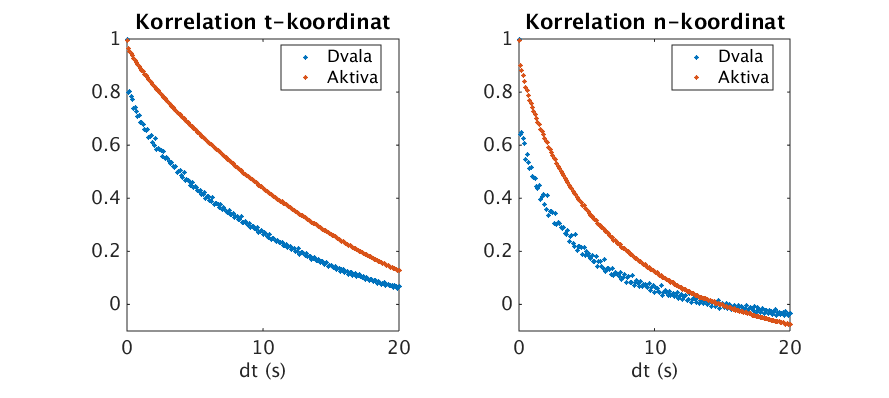
\includegraphics[width=.8\textwidth]{Korrelation_tnkoordinat.png}
    \caption{Korrelation i tangent- och normal-koordinaterna för aktiva celler och celler i dvala. I båda fall sjunker korrelationen initialt snabbare för cellerna i dvala. Korrelationen tycks även bestå längre i tangentialkoordinaten än normalkoordinaten vilket tyder på att det finns en föredragen väg.}
    \label{fig:Korr_tn}
\end{figure}

\paragraph{Avvikelse från brownsk rörelse}
%Har vi exempel på avvikelse från teorin kan dessa läggas under seprata underrubriker här
Utifrån teorin kring brownsk rörelse kan vissa förutsägelser göras för partiklar som strikt följer denna typ av rörelse. Bland annat räknades det fram i sektion \ref{sec:Brownsk} att mean square displacement (MSD) för en sådan partikel skulle öka linjärt med tiden, se ekvation \eqref{eq:MSD_Brownsk}. Utifrån givna data för arbetet har ett potenssamband kunnat anpassas med en exponent som är skilld från och betydligt lägre än 1. Detta tyder på att partikeln inte utför en ren brownsk rörelse utan genomgår en så kallad subdiffusion, karakteriserat att partikelns MSD beror av tiden via ett potenssamband med exponent mindre än 1 men större än 0.
\todo{Här kan bild infogas}

Vidare finns det minst två sätt att beräkna partiklarnas MSD. För stationära processer, dvs processer som inte explicit beror på när i tiden de inleds, kan man skapa ett medelvärde mellan alla möjliga mätpunkter separerade med givet tidsintervall så som beskrivet i ekvation ...
\todo{Kanske bör vi lägga till ett stycke om hur egenskaperna beräknas utifrån diskret data}
Genom att jämföra resultatet från denna typ av beräkning med att istället bara ta medelvärdet mellan alla partiklars kvadrerade radiella avvikelse från startpunkten vid given tid från start kan man avgöra om processen är stationär.
\todo{Bild för jämförelse mellan lilla och stora delta}
Båda dessa beräkningar har utförts för given data och exponentens värde i sambandet mellan MSD och tid skiljer sig/överensstämmer för lite för att någon tydlig slutsats hurvida processen är stationär eller ej ska kunna dras. \todo{Eller?}


\section{Diskussion och slutsats}







%Bara en liten kodsnutt som behövs när man kompilerar lokalt
%%% Local Variables: 
%%% mode: latex
%%% TeX-master: "main.tex"
%%% End: 